
\documentclass[conference]{IEEEtran}
\IEEEoverridecommandlockouts



% *** CITATION PACKAGES ***
%
\usepackage{cite}
% cite.sty was written by Donald Arseneau
% V1.6 and later of IEEEtran pre-defines the format of the cite.sty package
% \cite{} output to follow that of IEEE. Loading the cite package will
% result in citation numbers being automatically sorted and properly
% "compressed/ranged". e.g., [1], [9], [2], [7], [5], [6] without using
% cite.sty will become [1], [2], [5]--[7], [9] using cite.sty. cite.sty's
% \cite will automatically add leading space, if needed. Use cite.sty's
% noadjust option (cite.sty V3.8 and later) if you want to turn this off
% such as if a citation ever needs to be enclosed in parenthesis.
% cite.sty is already installed on most LaTeX systems. Be sure and use
% version 5.0 (2009-03-20) and later if using hyperref.sty.
% The latest version can be obtained at:
% http://www.ctan.org/tex-archive/macros/latex/contrib/cite/
% The documentation is contained in the cite.sty file itself.






% *** GRAPHICS RELATED PACKAGES ***
%
\ifCLASSINFOpdf
  % \usepackage[pdftex]{graphicx}
  % declare the path(s) where your graphic files are
  % \graphicspath{{../pdf/}{../jpeg/}}
  % and their extensions so you won't have to specify these with
  % every instance of \includegraphics
  % \DeclareGraphicsExtensions{.pdf,.jpeg,.png}
\else
  % or other class option (dvipsone, dvipdf, if not using dvips). graphicx
  % will default to the driver specified in the system graphics.cfg if no
  % driver is specified.
  % \usepackage[dvips]{graphicx}
  % declare the path(s) where your graphic files are
  % \graphicspath{{../eps/}}
  % and their extensions so you won't have to specify these with
  % every instance of \includegraphics
  % \DeclareGraphicsExtensions{.eps}
\fi
% graphicx was written by David Carlisle and Sebastian Rahtz. It is
% required if you want graphics, photos, etc. graphicx.sty is already
% installed on most LaTeX systems. The latest version and documentation
% can be obtained at: 
% http://www.ctan.org/tex-archive/macros/latex/required/graphics/
% Another good source of documentation is "Using Imported Graphics in
% LaTeX2e" by Keith Reckdahl which can be found at:
% http://www.ctan.org/tex-archive/info/epslatex/
%
% latex, and pdflatex in dvi mode, support graphics in encapsulated
% postscript (.eps) format. pdflatex in pdf mode supports graphics
% in .pdf, .jpeg, .png and .mps (metapost) formats. Users should ensure
% that all non-photo figures use a vector format (.eps, .pdf, .mps) and
% not a bitmapped formats (.jpeg, .png). IEEE frowns on bitmapped formats
% which can result in "jaggedy"/blurry rendering of lines and letters as
% well as large increases in file sizes.
%
% You can find documentation about the pdfTeX application at:
% http://www.tug.org/applications/pdftex





% *** MATH PACKAGES ***
%
%\usepackage[cmex10]{amsmath}
% A popular package from the American Mathematical Society that provides
% many useful and powerful commands for dealing with mathematics. If using
% it, be sure to load this package with the cmex10 option to ensure that
% only type 1 fonts will utilized at all point sizes. Without this option,
% it is possible that some math symbols, particularly those within
% footnotes, will be rendered in bitmap form which will result in a
% document that can not be IEEE Xplore compliant!
%
% Also, note that the amsmath package sets \interdisplaylinepenalty to 10000
% thus preventing page breaks from occurring within multiline equations. Use:
%\interdisplaylinepenalty=2500
% after loading amsmath to restore such page breaks as IEEEtran.cls normally
% does. amsmath.sty is already installed on most LaTeX systems. The latest
% version and documentation can be obtained at:
% http://www.ctan.org/tex-archive/macros/latex/required/amslatex/math/





% *** SPECIALIZED LIST PACKAGES ***
%
%\usepackage{algorithmic}
% algorithmic.sty was written by Peter Williams and Rogerio Brito.
% This package provides an algorithmic environment fo describing algorithms.
% You can use the algorithmic environment in-text or within a figure
% environment to provide for a floating algorithm. Do NOT use the algorithm
% floating environment provided by algorithm.sty (by the same authors) or
% algorithm2e.sty (by Christophe Fiorio) as IEEE does not use dedicated
% algorithm float types and packages that provide these will not provide
% correct IEEE style captions. The latest version and documentation of
% algorithmic.sty can be obtained at:
% http://www.ctan.org/tex-archive/macros/latex/contrib/algorithms/
% There is also a support site at:
% http://algorithms.berlios.de/index.html
% Also of interest may be the (relatively newer and more customizable)
% algorithmicx.sty package by Szasz Janos:
% http://www.ctan.org/tex-archive/macros/latex/contrib/algorithmicx/




% *** ALIGNMENT PACKAGES ***
%
%\usepackage{array}
% Frank Mittelbach's and David Carlisle's array.sty patches and improves
% the standard LaTeX2e array and tabular environments to provide better
% appearance and additional user controls. As the default LaTeX2e table
% generation code is lacking to the point of almost being broken with
% respect to the quality of the end results, all users are strongly
% advised to use an enhanced (at the very least that provided by array.sty)
% set of table tools. array.sty is already installed on most systems. The
% latest version and documentation can be obtained at:
% http://www.ctan.org/tex-archive/macros/latex/required/tools/


% IEEEtran contains the IEEEeqnarray family of commands that can be used to
% generate multiline equations as well as matrices, tables, etc., of high
% quality.




% *** SUBFIGURE PACKAGES ***
%\ifCLASSOPTIONcompsoc
%  \usepackage[caption=false,font=normalsize,labelfont=sf,textfont=sf]{subfig}
%\else
%  \usepackage[caption=false,font=footnotesize]{subfig}
%\fi
% subfig.sty, written by Steven Douglas Cochran, is the modern replacement
% for subfigure.sty, the latter of which is no longer maintained and is
% incompatible with some LaTeX packages including fixltx2e. However,
% subfig.sty requires and automatically loads Axel Sommerfeldt's caption.sty
% which will override IEEEtran.cls' handling of captions and this will result
% in non-IEEE style figure/table captions. To prevent this problem, be sure
% and invoke subfig.sty's "caption=false" package option (available since
% subfig.sty version 1.3, 2005/06/28) as this is will preserve IEEEtran.cls
% handling of captions.
% Note that the Computer Society format requires a larger sans serif font
% than the serif footnote size font used in traditional IEEE formatting
% and thus the need to invoke different subfig.sty package options depending
% on whether compsoc mode has been enabled.
%
% The latest version and documentation of subfig.sty can be obtained at:
% http://www.ctan.org/tex-archive/macros/latex/contrib/subfig/




% *** FLOAT PACKAGES ***
%
%\usepackage{fixltx2e}
% fixltx2e, the successor to the earlier fix2col.sty, was written by
% Frank Mittelbach and David Carlisle. This package corrects a few problems
% in the LaTeX2e kernel, the most notable of which is that in current
% LaTeX2e releases, the ordering of single and double column floats is not
% guaranteed to be preserved. Thus, an unpatched LaTeX2e can allow a
% single column figure to be placed prior to an earlier double column
% figure. The latest version and documentation can be found at:
% http://www.ctan.org/tex-archive/macros/latex/base/


%\usepackage{stfloats}
% stfloats.sty was written by Sigitas Tolusis. This package gives LaTeX2e
% the ability to do double column floats at the bottom of the page as well
% as the top. (e.g., "\begin{figure*}[!b]" is not normally possible in
% LaTeX2e). It also provides a command:
%\fnbelowfloat
% to enable the placement of footnotes below bottom floats (the standard
% LaTeX2e kernel puts them above bottom floats). This is an invasive package
% which rewrites many portions of the LaTeX2e float routines. It may not work
% with other packages that modify the LaTeX2e float routines. The latest
% version and documentation can be obtained at:
% http://www.ctan.org/tex-archive/macros/latex/contrib/sttools/
% Do not use the stfloats baselinefloat ability as IEEE does not allow
% \baselineskip to stretch. Authors submitting work to the IEEE should note
% that IEEE rarely uses double column equations and that authors should try
% to avoid such use. Do not be tempted to use the cuted.sty or midfloat.sty
% packages (also by Sigitas Tolusis) as IEEE does not format its papers in
% such ways.
% Do not attempt to use stfloats with fixltx2e as they are incompatible.
% Instead, use Morten Hogholm'a dblfloatfix which combines the features
% of both fixltx2e and stfloats:
%
% \usepackage{dblfloatfix}
% The latest version can be found at:
% http://www.ctan.org/tex-archive/macros/latex/contrib/dblfloatfix/




% *** PDF, URL AND HYPERLINK PACKAGES ***
%
%\usepackage{url}
% url.sty was written by Donald Arseneau. It provides better support for
% handling and breaking URLs. url.sty is already installed on most LaTeX
% systems. The latest version and documentation can be obtained at:
% http://www.ctan.org/tex-archive/macros/latex/contrib/url/
% Basically, \url{my_url_here}.

\usepackage{tikz}
\usetikzlibrary{shapes,arrows}
\usepackage{pgfplots}


% *** Do not adjust lengths that control margins, column widths, etc. ***
% *** Do not use packages that alter fonts (such as pslatex).         ***
% There should be no need to do such things with IEEEtran.cls V1.6 and later.
% (Unless specifically asked to do so by the journal or conference you plan
% to submit to, of course. )


% correct bad hyphenation here
\hyphenation{op-tical net-works semi-conduc-tor}


\begin{document}
%
% paper title
% Titles are generally capitalized except for words such as a, an, and, as,
% at, but, by, for, in, nor, of, on, or, the, to and up, which are usually
% not capitalized unless they are the first or last word of the title.
% Linebreaks \\ can be used within to get better formatting as desired.
% Do not put math or special symbols in the title.
\title{One Solution of the Accurate Summation \\ Using Fixed-point Accumulator}


\author{
	\thanks{
		This work was partially supported by the Ministry of Education, 
		Science and Technological Development of the Republic of Serbia, 
		under grant number: TR32031
	}
	Jelena Jankovic,\thanks{
		Jelena Jankovic is with the University of Novi Sad, Faculty of Technical sciences, 
		Computing and control engineering dept., 
		Trg Dositeja Obradovica 6, 21000 Novi Sad, Serbia
		(phone: 381-21-6623169; e-mail: jelenaa31051994@gmail.com)
	}
	Milos Subotic,\thanks{
		Milos Subotic is with RT-RK Institute for Computer Based Systems,
		Narodnog fronta 23a, 21000 Novi Sad, Serbia
		(phone: 381-21-4801291; e-mail: milos.subotic@rt-rk.com)
	}
	Vladimir Marinkovic\thanks{
		Vladimir Marinkovic is with RT-RK Institute for Computer based systems,
		Narodnog fronta 23a, 21000 Novi Sad, Serbia
		(phone: 381-21-4801291; e-mail: vladimir.marinkovic@rt-rk.com)
	}
}


\maketitle


\begin{abstract}
Accurate summation is algorithm for summing floating-point numbers with reduced rounding errors.
This paper presents one solution of accurate summation problem using fixed-point accumulator.
%TODO After we found out performances of algorithm choose one of those two sentances.
%In compare with other algorithms, solution has outperforming precision and comparable performances.
%In compare with other algorithms, solution has outperforming precision and performances.
\end{abstract}

\begin{IEEEkeywords}
Accurate summation, summation algorithm, floating-point numbers, fixed-point, rounding errors
\end{IEEEkeywords}




% For peer review papers, you can put extra information on the cover
% page as needed:
% \ifCLASSOPTIONpeerreview
% \begin{center} \bfseries EDICS Category: 3-BBND \end{center}
% \fi
%
% For peerreview papers, this IEEEtran command inserts a page break and
% creates the second title. It will be ignored for other modes.
\IEEEpeerreviewmaketitle


\section{Introduction}
% no \IEEEPARstart
Accurate summation \cite{Higham} is algorithm for summing floating-point numbers. 
It is well known that the summation of large sets of numbers can be very inaccurate due
to the accumulation of rounding errors. 
\par
One typical problem is one large, many small \cite{} 
where one big number is being summed with many small numbers. 
For example, in four digit decade floating-point space,
if 1000 small numbers 0.001 is accumulated to one large number 1.000, result would be 2.000. On the other hand,
if one large number 1.000 is summed with 1000 small numbers 0.001,
result would be 1.000 instead of 2.000 because of rounding errors.
\par
This paper


\section{Related work}
\label{sec:related_work}
% Could be like 2 sentences.
Several authors have used variety of methods for floating-point summation to find out which methods achieve the best accuracy. 
Methods that have been used are: 
\par
The first algorithm is Kahan's method \cite{Kahan}. This method uses additional variable in which rounding error of previous summation is carried to next one.
	\item Solution is  unique. In the world of Maxwell's equation scattered fields are 
		continuous function of the incident field and electromagnetic properties of object, 
		so solution will be unique if scattered fields are sampled in the
		all positions outside object and on all frequencies	\cite{ManitobaColinGilmorePhD}.
		Practically it is possible to record fields in finite number of points and frequencies.
	\item Stability. Small change in incident field could result in large change in scattered fields.
		Practically measured data is always corrupted by noise, which have great impact on stability.
\end{itemize}
Because of all these reasons inverse problems in microwave tomography are ill-posed.
\par
One important way for characterising microwave tomographic system is resolution.
Theoretically, after linearisation of inverse scattering problem and applying Rayleigh criteria
resolution \cite{TheoreticalSuperResolution} is limited to $\lambda / 2$ in the far-field 
and $\lambda / 4$ in the near-field, where $\lambda$ is wavelength, 
where border between near-field and far-field is practically $\lambda$ from wave source.
Experiments \cite{ManitobaSuperResolutionExperiment} show that even resolution of $\lambda / 30$ is obtainable,
which is phenomenon of the super-resolution.
Also it is suggested that resolution depends on signal-to-noise ratio \cite{ResolutionDependsOnNoise} rather than wavelength.
\par
Selection of working frequency is based on optimization resolution and wave penetration \cite{FrequencySelection}.
Systems with higher frequencies have better resolution, but because of higher attenuation penetration of waves is smaller.
If it is true that resolution depends only on signal-to-noise ratio then well designed near-field lower frequency system 
could observe larger objects.
%TODO Find ref where we read that near-field don't have Fraunhoffer difraction as a far-field
% which is the one main of problems with resolution on far-field, 
% and if remeber good why super-resolution exists and Rayleigh's limit doesn't work on near-field, 
% and then state that here.
\par
This work recognizes problem of non-uniqueness when imaging objects in the far-field, 
as it will be seen in next section,
and additionally promote near-field.



\section{Problem}
\label{sec:problem}
In Fig.~\ref{fig:ambiguous_situation} is shown ambiguous situation in 1D space,
which occurs when object of interest is observed in far-field of the waves.
Figure depict two simplified diagrams of real situation where 
object of interest (shaded region) is observed in background media.
On this diagrams point $A$ is source 
of the incident excitation EM waves represented by filled line,
measurement of reflected dotted wave is done point $A$,
and measurement of transmitted dashed wave is done $B$. 
Difference between these two diagrams is that object in second is moved
for half of wavelength in the background media.
It could be seen that reflected and transmitted waves are of the same 
magnitude and phase in the points $A$ and $B$ on the both cases,
so moving object for half of wavelength could not be detected.
Same could be concluded for moving object 
for any integer multiply of half of wavelength.

\begin{figure}[!t]
	\centering
    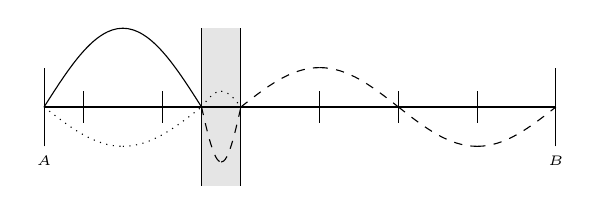
\begin{tikzpicture}
		\fill[black!10] (2, -1) rectangle (2.5, 1);
		
		\draw (0,0) -- (6.5,0);

		\draw (0, -0.5) node [below,font=\tiny] {$A$} -- (0, 0.5);
		\foreach \x in {0.5,1.5,...,6.0}{
			\draw (\x, -0.2) node {} -- (\x, 0.2);
		}
		\draw (6.5, -0.5) node [below,font=\tiny] {$B$} -- (6.5, 0.5);
		
		\draw(2, -1) node {} -- (2, 1);
		\draw(2.5, -1) node {} -- (2.5, 1);
		
		\draw[] (0, 0) sin (1, 1);
		\draw[] (1, 1) cos (2, 0);
		
		\draw[dashed] (2, 0) sin (2.25, -0.7);
		\draw[dashed] (2.25, -0.7) cos (2.5, 0);
		\draw[dotted] (2, 0) sin (2.25, 0.2);
		\draw[dotted] (2.25, 0.2) cos (2.5, 0);
		
		\draw[dashed] (2.5, 0) sin (3.5, 0.5);
		\draw[dashed] (3.5, 0.5) cos (4.5, 0);
		\draw[dashed] (4.5, 0) sin (5.5, -0.5);
		\draw[dashed] (5.5, -0.5) cos (6.5, 0);

		\draw[dotted] (0, 0) sin (1, -0.5);
		\draw[dotted] (1, -0.5) cos (2, 0);
		
	\end{tikzpicture}
	
    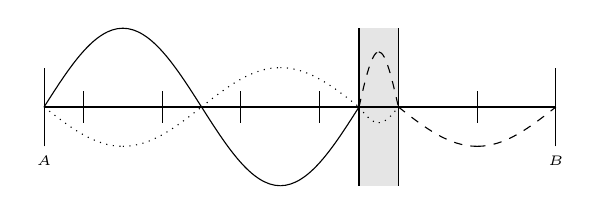
\begin{tikzpicture}    
		\fill[black!10] (4, -1) rectangle (4.5, 1);
		
		\draw (0,0) -- (6.5,0);

		\draw (0, -0.5) node [below,font=\tiny] {$A$} -- (0, 0.5);
		\foreach \x in {0.5,1.5,...,6.0}{
			\draw (\x, -0.2) node {} -- (\x, 0.2);
		}
		\draw (6.5, -0.5) node [below,font=\tiny] {$B$} -- (6.5, 0.5);
		
		\draw(4, -1) node {} -- (4, 1);
		\draw(4.5, -1) node {} -- (4.5, 1);
				
		\draw[] (0, 0) sin (1, 1);
		\draw[] (1, 1) cos (2, 0);
		\draw[] (2, 0) sin (3, -1);
		\draw[] (3, -1) cos (4, 0);
		
		\draw[dashed] (4, 0) sin (4.25, 0.7);
		\draw[dashed] (4.25, 0.7) cos (4.5, 0);
		\draw[dotted] (4, 0) sin (4.25, -0.2);
		\draw[dotted] (4.25, -0.2) cos (4.5, 0);
		
		\draw[dashed] (4.5, 0) sin (5.5, -0.5);
		\draw[dashed] (5.5, -0.5) cos (6.5, 0);

		\draw[dotted] (0, 0) sin (1, -0.5);
		\draw[dotted] (1, -0.5) cos (2, 0);
		\draw[dotted] (2, 0) sin (3, 0.5);
		\draw[dotted] (3, 0.5) cos (4, 0);
		
	\end{tikzpicture}	
	
	\caption{Ambiguous situation in 1D}
	\label{fig:ambiguous_situation}
\end{figure}

\par
Same problem could be generalized for 2D and 3D space.
%TODO Maybe diagram if need more pages.


\par
This ambiguous situations could be one reason for non-uniqueness,
typical for inverse problems.
Additional observation points could help solving this problem.
For situation in Fig.~\ref{fig:ambiguous_situation} adding measurement point
in-between two object position could eliminate ambiguity.
Also problem could be solved by frequency-hopping method \cite{FrequencyHopping} i.e. 
illuminating object with multiple frequencies. 
It is important to notice that these frequencies have to be of non-integer ratio.
For example doubled frequency will still produce ambiguity,
and half frequency will make ambiguity two time less often.
Another technique to cope with this problem are multiple excitation points.
%TODO This sentence need diagram: Same stands for 2D example, and futher on 3D.
Insufficient number of observation points and frequencies
are the main reason of non-uniqueness of solution
and ill-posedness of inverse problem \cite{ManitobaColinGilmorePhD},
as depicted in Section~\ref{sec:related_work}.


\section{Experimental results}
Existence of ambiguous situation is proven by numerical experiments.
For forward solver we use Finite-Difference Time-Domain (FDTD) \cite{FDTDbible},
numerical algorithm for simulating electromagnetic waves propagation in time domain.
In contrast to frequency domain methods FDTD work with multiple frequencies,
so it is easy to implement frequency-hopping methods.
Also FDTD enables direct visualisation of real E and H fields in space,
which gives great insights in the problem.
Experiments are implemented with 1D FDTD with Perfect Boundary Condition (PBC) 
and numeric dispersion compensation. % This is only for experts.
Forward solver is used as model to generate target fields from the target dielectric map,
which acts as a measured fields data in real system.
After that we visualise fitness between guessed and target fields,
or do the Particle Swarm Optimization (PSO) \cite{SecondOldestPSOPaper} algorithm
to find best fit to target dielectric map.
Fitness is calculated from FFT of fields in one or multiple frequencies (frequency-hopping).
\par
Good way for researching non-uniqueness is visualization of the fitness.
1D FDTD simulation with both objects from Fig.~\ref{fig:ambiguous_situation} is made.
Objects are at distance $\lambda/2$.
We simulate only dielectric characteristics of materials i.e. relative permittivity $\epsilon_r$.
Background media $\epsilon_r = 1$.
For visualization only two dimensions are chosen,
which are $\epsilon_{r0}$ and $\epsilon_{r1}$, relative permittivity of two objects.
If one object have same $\epsilon_r$ as background media i.e. 1, 
then it is equivalent to situation where it does not exists.
In target situation for first and second object we have for example
$\epsilon_{r0} = 2.5$ and $\epsilon_{r1} = 1.0$.
Ambiguous situation would be $\epsilon_{r0} = 1.0$ and $\epsilon_{r1} = 2.5$.
We visualize all object sizes up to $\lambda/2$.
3D plot with $\epsilon_{r0}$ and $\epsilon_{r1}$ 
for $x$ and $y$ axes and fitness for $z$ axis could be unclear,
so we illustrate on 2D plot only fitness along the diagonal which pass through 
target point ($\epsilon_{r0} = 2.5$ and $\epsilon_{r1} = 1.0$) 
and ambiguous point ($\epsilon_{r0} = 1.0$ and $\epsilon_{r1} = 2.5$).
This is illustrated in Figures \ref{fig:fitness12} and \ref{fig:fitness13}.



\begin{figure}[!t]
	\centering
	
	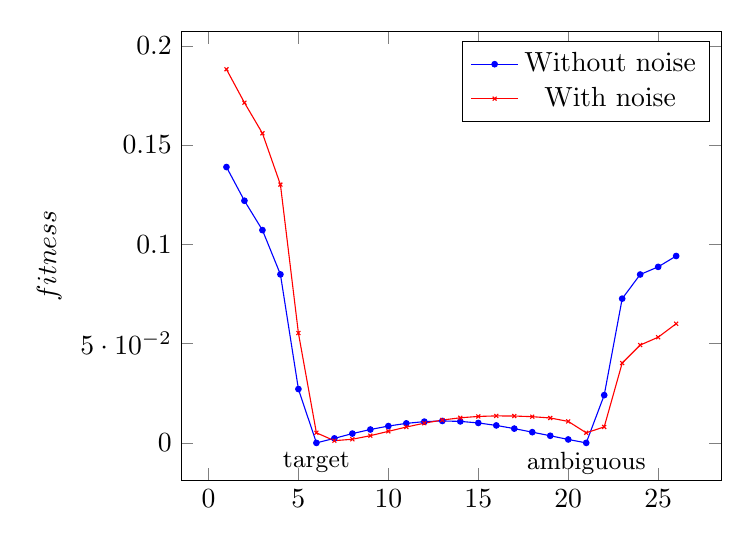
\begin{tikzpicture}
		\begin{axis}[
			ylabel=$fitness$
		]
			\addplot[mark size=1pt,mark=*,blue] plot coordinates {
				(1, 0.138942)
				(2, 0.121965)
				(3, 0.107172)
				(4, 0.084873)
				(5, 0.0271228)
				(6, 0)
				(7, 0.00227543)
				(8, 0.00468809)
				(9, 0.00673579)
				(10, 0.0084736)
				(11, 0.0098297)
				(12, 0.0107114)
				(13, 0.0110511)
				(14, 0.010822)
				(15, 0.0100453)
				(16, 0.00879377)
				(17, 0.00719193)
				(18, 0.0054046)
				(19, 0.00358632)
				(20, 0.00172819)
				(21, 1.14092e-30)
				(22, 0.0240487)
				(23, 0.0726431)
				(24, 0.0848067)
				(25, 0.0886562)
				(26, 0.0941337)
			};
			\addlegendentry{Without noise}

			\addplot[mark size=1pt,mark=x,color=red] plot coordinates {
				(1, 0.188175)
				(2, 0.171345)
				(3, 0.155934)
				(4, 0.130099)
				(5, 0.0553202)
				(6, 0.00508105)
				(7, 0.00110905)
				(8, 0.00182746)
				(9, 0.0036362)
				(10, 0.00580916)
				(11, 0.00798442)
				(12, 0.00993212)
				(13, 0.0115092)
				(14, 0.0126432)
				(15, 0.0133227)
				(16, 0.01359)
				(17, 0.0135252)
				(18, 0.0132018)
				(19, 0.0125418)
				(20, 0.0108133)
				(21, 0.00508105)
				(22, 0.0080297)
				(23, 0.0402093)
				(24, 0.0492598)
				(25, 0.053229)
				(26, 0.0600298)
			};
			\addlegendentry{With noise}
			
			\pgfplotsset{
				after end axis/.code={
					\node[below] at (axis cs:6,0){\small{target}};
					\node[below] at (axis cs:21,0){\small{ambiguous}};
				}
			}
		\end{axis}
	\end{tikzpicture}
	
	\caption{Fitness diagonal for objects size $\frac{12}{20}\frac{\lambda}{2}$}
	\label{fig:fitness12}
\end{figure}

\begin{figure}[!t]
	\centering
	
	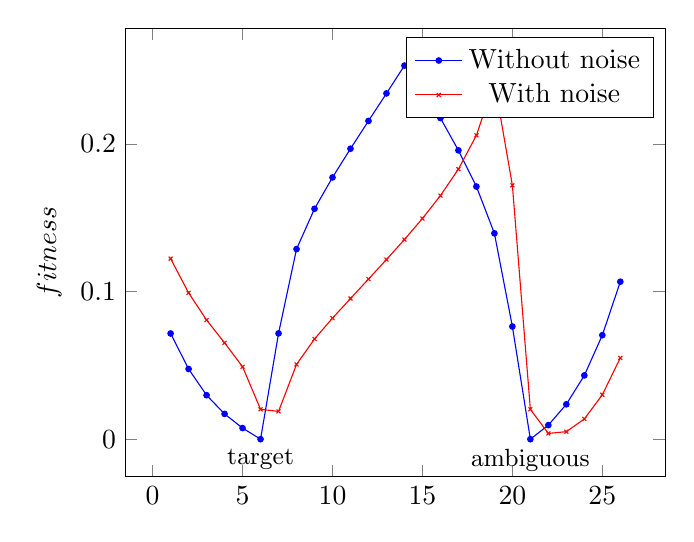
\begin{tikzpicture}
		\begin{axis}[
			ylabel=$fitness$
		]
			\addplot[mark size=1pt,mark=*,blue] plot coordinates {
				(1, 0.0716105)
				(2, 0.0475529)
				(3, 0.0297978)
				(4, 0.0171223)
				(5, 0.00753355)
				(6, 0)
				(7, 0.0716663)
				(8, 0.128782)
				(9, 0.15608)
				(10, 0.177323)
				(11, 0.196773)
				(12, 0.215585)
				(13, 0.234231)
				(14, 0.253071)
				(15, 0.238137)
				(16, 0.217519)
				(17, 0.195644)
				(18, 0.17114)
				(19, 0.139448)
				(20, 0.0763078)
				(21, 5.22422e-31)
				(22, 0.00953318)
				(23, 0.023632)
				(24, 0.0431994)
				(25, 0.0704558)
				(26, 0.106667)
			};
			\addlegendentry{Without noise}

			\addplot[mark size=1pt,mark=x,color=red] plot coordinates {
				(1, 0.122312)
				(2, 0.0991312)
				(3, 0.0807121)
				(4, 0.0652672)
				(5, 0.0490707)
				(6, 0.0202285)
				(7, 0.0188214)
				(8, 0.0506484)
				(9, 0.0678895)
				(10, 0.0819844)
				(11, 0.095294)
				(12, 0.108443)
				(13, 0.121688)
				(14, 0.135255)
				(15, 0.149489)
				(16, 0.164994)
				(17, 0.182913)
				(18, 0.205834)
				(19, 0.242068)
				(20, 0.171955)
				(21, 0.0202285)
				(22, 0.00389591)
				(23, 0.00509795)
				(24, 0.0136965)
				(25, 0.0300729)
				(26, 0.0550486)

			};
			\addlegendentry{With noise}
			
			\pgfplotsset{
				after end axis/.code={
					\node[below] at (axis cs:6,0){\small{target}};
					\node[below] at (axis cs:21,0){\small{ambiguous}};
				}
			}
		\end{axis}
	\end{tikzpicture}
	
	\caption{Fitness diagonal for objects size $\frac{13}{20}\frac{\lambda}{2}$}
	\label{fig:fitness13}
\end{figure}

\par
From Figures \ref{fig:fitness12} and \ref{fig:fitness13} 
it could be seen that fitnesses without noise have two minimums, 
target and ambiguous, with almost same very small value.
Optimization algorithm, which is stochastic by design,
will sometimes converge to target and sometimes to ambiguous minimum,
and sometimes give wrong result for $\epsilon_{r0}$ and $\epsilon_{r1}$
\par
When running experiments with simulated noise in measured data 
ambiguous minimum could become higher than target minimum become local minimum,
as depicted in Fig.~\ref{fig:fitness12}.
In this situation, setting higher optimization algorithm threshold 
(higher than local ambiguous minimum)
will make optimization algorithm to always converge to correct target minimum.
Even if ambigiuous minimum is higher that target minimum,
it will still make impact on optimization algorithm performance 
because it is huge local minimum.
\par
Also target minimum could become higher than ambiguous,
so ambiguous minimum will better fit than target,
as depicted in Fig.~\ref{fig:fitness13}.
In this situation optimization algorithm will always converge to wrong ambiguous minimum.

\begin{figure}[!t]
	\centering
	
	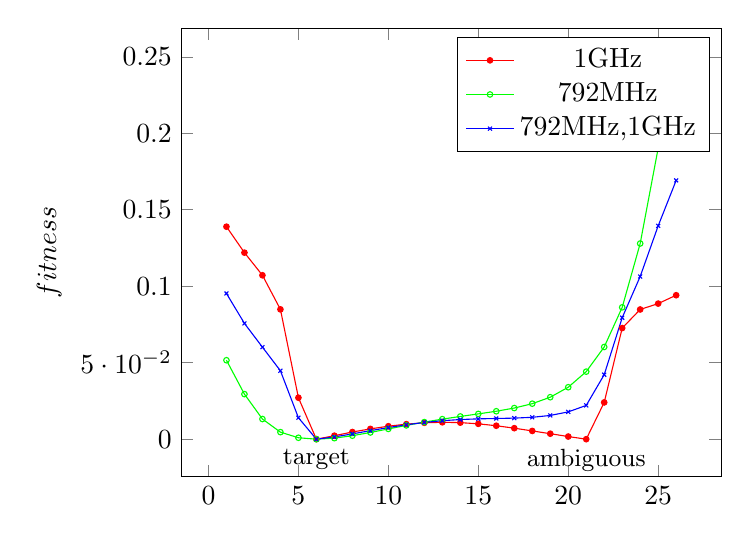
\begin{tikzpicture}
		\begin{axis}[
			ylabel=$fitness$
		]
			\addplot[mark size=1pt,mark=*,red] plot coordinates {
				(1, 0.13894170451490703)
				(2, 0.12196510598570702)
				(3, 0.10717164479820254)
				(4, 0.08487304400995402)
				(5, 0.02712282142808604)
				(6, 0.0)
				(7, 0.002275429664558802)
				(8, 0.004688085542797045)
				(9, 0.006735790148544309)
				(10, 0.008473600130367848)
				(11, 0.009829699280764296)
				(12, 0.010711426535362148)
				(13, 0.011051065384836701)
				(14, 0.010821972761173627)
				(15, 0.01004530348680362)
				(16, 0.008793769617181722)
				(17, 0.007191925598700502)
				(18, 0.005404597594628852)
				(19, 0.003586321969123592)
				(20, 0.0017281949554771164)
				(21, 1.1409201179205967e-30)
				(22, 0.024048685919716515)
				(23, 0.07264310395259808)
				(24, 0.08480670466616111)
				(25, 0.08865616647741148)
				(26, 0.09413371732531627)
			};
			\addlegendentry{1GHz}

			\addplot[mark size=1pt,mark=o,color=green] plot coordinates {
				(1, 0.05161517232960979)
				(2, 0.02945377228405059)
				(3, 0.013179784365634885)
				(4, 0.004599593806473532)
				(5, 0.0009346605588960757)
				(6, 0.0)
				(7, 0.0006649261080062096)
				(8, 0.0022767370290914064)
				(9, 0.004396318353091135)
				(10, 0.006712469876183653)
				(11, 0.009011574413065462)
				(12, 0.011162994313195623)
				(13, 0.013110750026057976)
				(14, 0.014870278336124572)
				(15, 0.016531080518328398)
				(16, 0.018266772744267273)
				(17, 0.020354959075863956)
				(18, 0.02321131522748513)
				(19, 0.02744679245707121)
				(20, 0.03396767672533175)
				(21, 0.044164427822392965)
				(22, 0.06029186243507987)
				(23, 0.08619218591570658)
				(24, 0.12793583341969736)
				(25, 0.1902737196745197)
				(26, 0.24426947220538897)
			};
			\addlegendentry{792MHz}
			
			\addplot[mark size=1pt,mark=x,color=blue] plot coordinates {
				(1, 0.09527843842225842)
				(2, 0.0757094391348788)
				(3, 0.06017571458191871)
				(4, 0.04473631890821377)
				(5, 0.014028740993491058)
				(6, 0.0)
				(7, 0.0014701778862825057)
				(8, 0.0034824112859442257)
				(9, 0.005566054250817722)
				(10, 0.007593035003275751)
				(11, 0.009420636846914878)
				(12, 0.010937210424278886)
				(13, 0.012080907705447338)
				(14, 0.012846125548649098)
				(15, 0.013288192002566009)
				(16, 0.013530271180724498)
				(17, 0.01377344233728223)
				(18, 0.01430795641105699)
				(19, 0.015516557213097401)
				(20, 0.017847935840404432)
				(21, 0.022082213911196483)
				(22, 0.042170274177398194)
				(23, 0.07941764493415233)
				(24, 0.10637126904292923)
				(25, 0.13946494307596558)
				(26, 0.16920159476535263)
			};
			\addlegendentry{792MHz,1GHz}
			
			\pgfplotsset{
				after end axis/.code={
					\node[below] at (axis cs:6,0){\small{target}};
					\node[below] at (axis cs:21,0){\small{ambiguous}};
				}
			}
		\end{axis}
	\end{tikzpicture}
	
	\caption{Frequency-hopping fitness diagonals for objects size $\frac{12}{20}\frac{\lambda}{2}$}
	\label{fig:poly12}
\end{figure}

\begin{figure}[!t]
	\centering
	
	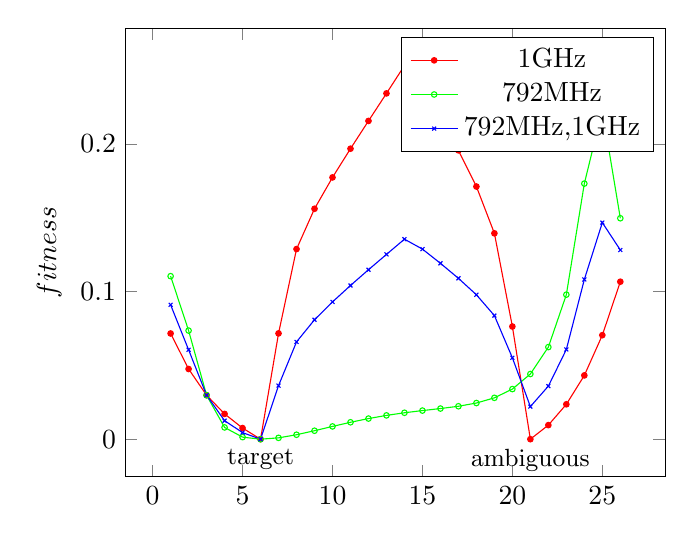
\begin{tikzpicture}
		\begin{axis}[
			ylabel=$fitness$
		]
			\addplot[mark size=1pt,mark=*,red] plot coordinates {
				(1, 0.0716105450168973)
				(2, 0.04755292762874107)
				(3, 0.029797847743561572)
				(4, 0.017122344465417456)
				(5, 0.0075335467590383915)
				(6, 0.0)
				(7, 0.07166631628207824)
				(8, 0.12878244037153244)
				(9, 0.15608048456643653)
				(10, 0.17732298000861477)
				(11, 0.1967728007869228)
				(12, 0.2155850789235749)
				(13, 0.23423115332415592)
				(14, 0.253070563534331)
				(15, 0.23813722322579645)
				(16, 0.21751858767607785)
				(17, 0.19564428199240622)
				(18, 0.171139980920678)
				(19, 0.13944831097521646)
				(20, 0.07630780429139754)
				(21, 5.224220043867002e-31)
				(22, 0.009533175504096495)
				(23, 0.023631964340618677)
				(24, 0.043199379719237825)
				(25, 0.07045581479453868)
				(26, 0.10666734428361298)
			};
			\addlegendentry{1GHz}

			\addplot[mark size=1pt,mark=o,color=green] plot coordinates {
				(1, 0.11043401728303326)
				(2, 0.07356477596946771)
				(3, 0.029775638054792622)
				(4, 0.00796785735217144)
				(5, 0.0013932287184793284)
				(6, 0.0)
				(7, 0.0008989462699526061)
				(8, 0.003017582077017381)
				(9, 0.005739466848219514)
				(10, 0.00864499349624998)
				(11, 0.011447542817487794)
				(12, 0.01396750232352638)
				(13, 0.016117342790660995)
				(14, 0.01789409137270598)
				(15, 0.0193797637410073)
				(16, 0.02075145165932095)
				(17, 0.022304189379463584)
				(18, 0.024493179281372124)
				(19, 0.028011319423447055)
				(20, 0.03394628161215542)
				(21, 0.044157639949182405)
				(22, 0.062379316211858465)
				(23, 0.09790010015636891)
				(24, 0.17313729856971435)
				(25, 0.22296303127290287)
				(26, 0.1496607443930434)
			};
			\addlegendentry{792MHz}
			
			\addplot[mark size=1pt,mark=x,color=blue] plot coordinates {
				(1, 0.09102228114996527)
				(2, 0.06055885179910439)
				(3, 0.0297867428991771)
				(4, 0.012545100908794448)
				(5, 0.00446338773875886)
				(6, 0.0)
				(7, 0.03628263127601542)
				(8, 0.06590001122427491)
				(9, 0.08090997570732802)
				(10, 0.09298398675243237)
				(11, 0.1041101718022053)
				(12, 0.11477629062355064)
				(13, 0.12517424805740845)
				(14, 0.1354823274535185)
				(15, 0.12875849348340188)
				(16, 0.1191350196676994)
				(17, 0.1089742356859349)
				(18, 0.09781658010102506)
				(19, 0.08372981519933176)
				(20, 0.05512704295177648)
				(21, 0.022078819974591202)
				(22, 0.03595624585797748)
				(23, 0.06076603224849379)
				(24, 0.10816833914447609)
				(25, 0.14670942303372078)
				(26, 0.12816404433832818)
			};
			\addlegendentry{792MHz,1GHz}
			
			\pgfplotsset{
				after end axis/.code={
					\node[below] at (axis cs:6,0){\small{target}};
					\node[below] at (axis cs:21,0){\small{ambiguous}};
				}
			}
		\end{axis}
	\end{tikzpicture}
	
	\caption{Frequency-hopping fitness diagonals for objects size $\frac{13}{20}\frac{\lambda}{2}$}
	\label{fig:poly13}
\end{figure}

\begin{figure}[!t]
	\centering
	
	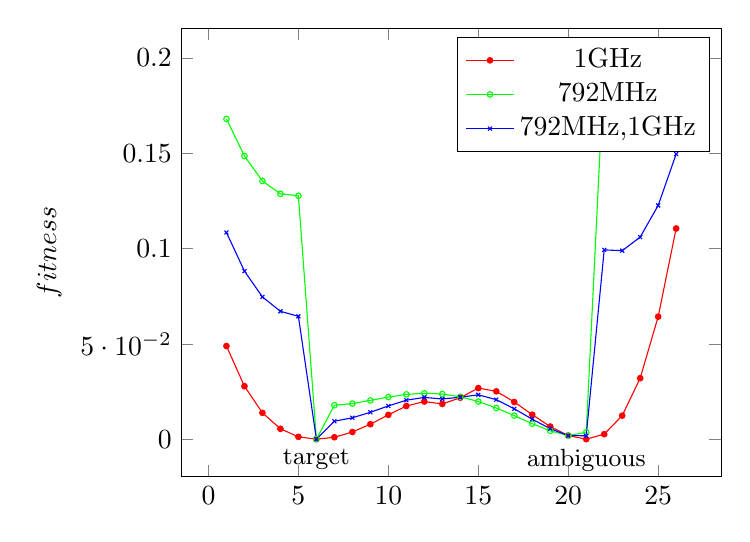
\begin{tikzpicture}
		\begin{axis}[
			ylabel=$fitness$
		]
			\addplot[mark size=1pt,mark=*,red] plot coordinates {
				(1, 0.04884356497412411)
				(2, 0.02778430517917658)
				(3, 0.013810574826726535)
				(4, 0.0054530913460679245)
				(5, 0.0012230059694920846)
				(6, 0.0)
				(7, 0.001018426979429192)
				(8, 0.0037707934084613513)
				(9, 0.007858072146006636)
				(10, 0.012749136612325608)
				(11, 0.01739524775428101)
				(12, 0.019744990353563998)
				(13, 0.018493181916180074)
				(14, 0.021749885262995677)
				(15, 0.026799925443525108)
				(16, 0.02510454556566331)
				(17, 0.019512918994027868)
				(18, 0.012845857023004418)
				(19, 0.0066242265583203955)
				(20, 0.001926847119753691)
				(21, 6.1422227072647e-29)
				(22, 0.002642587333987016)
				(23, 0.012335307774044752)
				(24, 0.03198683433569483)
				(25, 0.06425857920443405)
				(26, 0.11050116056876777)
			};
			\addlegendentry{1GHz}

			\addplot[mark size=1pt,mark=o,color=green] plot coordinates {
				(1, 0.1679281276237033)
				(2, 0.14851408167463465)
				(3, 0.13540847247820345)
				(4, 0.12867009562957882)
				(5, 0.12763470485895861)
				(6, 0.0)
				(7, 0.017813029272360382)
				(8, 0.018675842201891155)
				(9, 0.020344198258798463)
				(10, 0.022118095715781837)
				(11, 0.023478688059639943)
				(12, 0.02407361213173232)
				(13, 0.023691631264242397)
				(14, 0.022243636051244162)
				(15, 0.01975425811606326)
				(16, 0.016365363453016087)
				(17, 0.012351377278120005)
				(18, 0.008145062989411506)
				(19, 0.004369860715865195)
				(20, 0.0018704342659916619)
				(21, 0.0035978629445835818)
				(22, 0.19592202594630787)
				(23, 0.1853404564948036)
				(24, 0.179990813287986)
				(25, 0.18090351722294318)
				(26, 0.1885223671571214)
			};
			\addlegendentry{792MHz}
			
			\addplot[mark size=1pt,mark=x,color=blue] plot coordinates {
				(1, 0.10838584629891371)
				(2, 0.08814919342690561)
				(3, 0.074609523652465)
				(4, 0.06706159348782337)
				(5, 0.06442885541422536)
				(6, 0.0)
				(7, 0.009415728125894788)
				(8, 0.011223317805176252)
				(9, 0.01410113520240255)
				(10, 0.01743361616405372)
				(11, 0.020436967906960476)
				(12, 0.021909301242648158)
				(13, 0.021092406590211235)
				(14, 0.021996760657119918)
				(15, 0.023277091779794184)
				(16, 0.0207349545093397)
				(17, 0.015932148136073937)
				(18, 0.010495460006207963)
				(19, 0.005497043637092795)
				(20, 0.0018986406928726764)
				(21, 0.0017989314722917909)
				(22, 0.09928230664014744)
				(23, 0.09883788213442418)
				(24, 0.10598882381184041)
				(25, 0.12258104821368862)
				(26, 0.14951176386294457)
			};
			\addlegendentry{792MHz,1GHz}
			
			\pgfplotsset{
				after end axis/.code={
					\node[below] at (axis cs:6,0){\small{target}};
					\node[below] at (axis cs:21,0){\small{ambiguous}};
				}
			}
		\end{axis}
	\end{tikzpicture}
	
	\caption{Frequency-hopping fitness diagonals for objects size $\frac{16}{20}\frac{\lambda}{2}$}
	\label{fig:poly16}
\end{figure}

\par
Experiments shows that frequency-hopping method does not completely eliminate ill-posedness in the far-field.
In Fig.~\ref{fig:poly12} could be seen that two frequencies completely removed local minimum.
A little larger objects size local minimum shows up, as depicted in Fig.~\ref{fig:poly13}.
In Fig.~\ref{fig:poly16} ambiguous local minimum is significant.
Larger number of frequencies soften local minimums.
In practice, Ultra Wideband (UWB) \cite{UWBbible} EM waves are used for excitation,
to cover as many as possible frequencies.

\par
These experiments does not proof that near-field inverse problem is always well-posed,
but rather recognize one of the reasons of ill-posedness in the far-field.
These initial results encourage that toward thesis that
near-field imaging is less ill-posed than a far-field.
For proving this additional research have to be done to measure 
ill-posedness between near-field and the far-field.
If measure of ill-posedness is smaller
techniques for fighting ill-posedness mentioned in Section~\ref{sec:problem},
like frequency-hopping and larger number of observation point,
could be less applied or completely avoided.
That could simplify microwave tomography system.
\par
This experimental setup is corner case of the problems met in practice.
Usually objects under microwave tomography imaging would certainly have resistance 
and other electromagnetic characteristics.
Also this is 1D problem and almost all real problems are 2D or 3D.
This imply that additional experimentation is needed.


\section{Conclusion}
This paper recognize and proof impact of one of the possible cause of solution non-uniqueness 
and ill-posedness of inverse problem in microwave tomography,
when imaging objects in the far-field.
This does not proof that near-field imaging is always well-posed,
but rather opens discussion for compromise between near-field and the far-field imaging.
\par
Future work will be focused on the measuring ill-posedness 
between near-field and the far-field imaging.
One possible metric could be effort of optimization algorithm 
to find target dielectric map for given fitness.
Future research will also consider resolution of resulting images and wave penetration,
which are closely connected with ill-posedness of inverse problems in microwave tomography.


% use section* for acknowledgment
\section*{Acknowledgment}
This work was partially supported by the Ministry of Education, 
Science and Technological Development of the Republic of Serbia, 
under grant number: TR32031




\bibliographystyle{IEEEtran}
\bibliography{cites}


\end{document}
